\section{Experiment} \label{sec:experiment}

In this section, we evaluate our algorithms presented in the previous sections. We profile the GPU memory usage when training two linear feedforward DNN models with the optimal checkpoint subset returned by the algorithms. We do the same for comparison by profiling the training of the same models with non-optimal checkpoint subsets. Finally, we run the algorithm implementation of Feng et al.~\cite{feng2021optimal} to find and compare the differences between their works and ours.


\subsection{Environment Settings}

\subsubsection{Models and Definitions}

We use VGG-19~\cite{Simonyan2014VeryDC} and AlexNet~\cite{krizhevsky2017imagenet} as our DNN model to evaluate our algorithm.
VGG-19 has 16 convolution layers and 5 max-pooling layers, and 3 fully connected layers.
AlexNet has 5 convolution layers and 3 max-pooling layers, and 3 fully connected layers.

We define the term {\em training phase index} to describe every stage of training, including both the forward and backward phases. It is a number ranging from 0 to $2N+1$, where $N$ is the number of layers of the model. The value $0$ represents the stage before the training, and $2N+1$ represents the stage after training.
The training is in the forward phase when $i$ is in the range $1 \leq i \leq N$, and it is in the backward phase when $i$ is in the range $N+1 \leq i \leq 2N$. Now we can index the entire training.
Notice that we always measure the GPU memory at the end of every stage. For ease of index calculation, we do not merge the forward phase and the backward phase of the last layer.
Figures~\ref{fig:vgg19_layers} and \ref{fig:alexnet_layers} depict the training phase indices for VGG-19 and AlexNet, respectively. For example, the training phase index 29 of VGG-19 means that it is the stage in the backward phase of the 20th layer, i.e. we are in the backward phase of the last convolutional layer with 512 output channels.

\begin{figure}[h!]
    \centering
    \includegraphics[width=\textwidth]{Fig/vgg19_layers.pdf}
    \caption{Training phase indices of VGG-19.} 
    \label{fig:vgg19_layers}
\end{figure}
\begin{figure}[h!]
    \centering
    \includegraphics[width=.7\textwidth]{Fig/alexnet_layers.pdf}
    \caption{Training phase indices of AlexNet.} 
    \label{fig:alexnet_layers}
\end{figure}

\subsubsection{Benchmarks}

%We use ImageNet~\cite{russakovsky2015imagenet} and TinyImageNet to evaluate our algorithm.
%ImageNet consists of around 1.3 million color images of different sizes in 1000 classes.
%TinyImageNet~ consists of 0.1 million color images of the same size (64 by 64) in 200 classes.

%For ImageNet, we will crop all images into size 224 by 224 before feeding them into our model.

We use ImageNet~\cite{russakovsky2015imagenet} to evaluate our algorithms.
ImageNet consists of around 1.3 million color images of different sizes in 1000 classes.
We crop all images into size 224 by 224 before feeding them into the model.

\subsubsection{Implementation}

We use PyTorch~\cite{paszke2019pytorch} deep learning platform to implement the two DNN models VGG-19 and AlexNet.
To implement the recomputing of a segment in the checkpoint technique, we use the PyTorch API \texttt{torch.utils.checkpoint}.
To profile the GPU memory usage, we use the PyTorch API \texttt{torch.cuda.memory\_allocated}.
We include the fully-connected layers of both VGG-19 and AlexNet when selecting the candidate of checkpoints, in addition to convolution layers. 
This is because the memory cost of fully-connected layers is large.
Additionally, we exclude the layers of AdaptiveAvgPool2d, Flatten, and Dropout in VGG-19, but include these layers as checkpoint candidates in AlexNet.
This simplifies the selection of checkpoints for the $O(\sqrt{n})$ algorithm~\cite{chen2016training}.
We perform all experiments with GPUs of the same specs, NVIDIA GeForce RTX 3090, 24 GiB memory on a server with 16-core, 2.90 GHz Intel Xeon Gold 6226R CPU, 192 GiB RAM.


\subsection{Algorithm Prediction versus PyTorch Report} \label{sec:prediction}

In this experiment, we demonstrate the importance of the consideration of the output gradient buffer as we have mentioned in section~\ref{sec:dynamic_checkpoint}. We show that the prediction of GPU memory usage by our algorithm is aligned with the report from PyTorch.

\begin{figure}[h!t]
    \centering
    % This file was created with tikzplotlib v0.10.1.
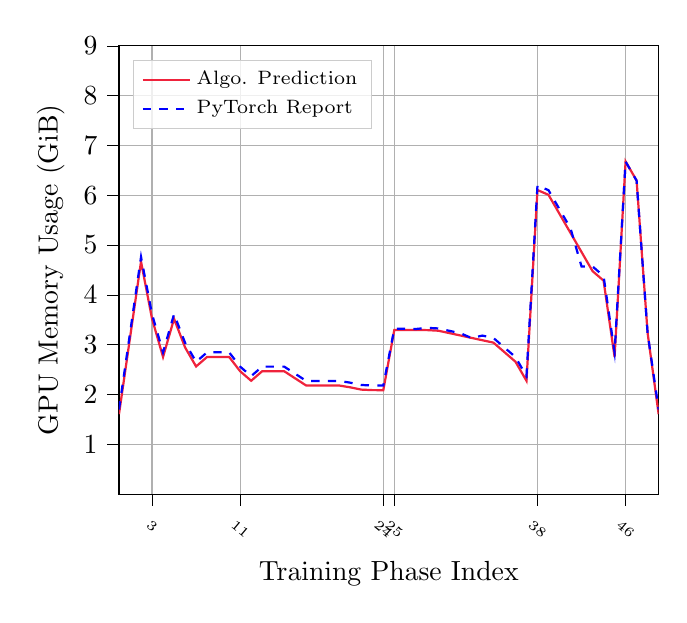
\begin{tikzpicture}

\definecolor{crimson2393560}{RGB}{239,35,60}
\definecolor{darkgray176}{RGB}{176,176,176}
\definecolor{lightgray204}{RGB}{204,204,204}

\begin{axis}[
legend cell align={left},
legend style={fill opacity=0.8, draw opacity=1, text opacity=1, draw=lightgray204},
tick align=outside,
tick pos=left,
title={ },
x grid style={darkgray176},
xlabel={Training Phase Index},
xmajorgrids,
xmin=0, xmax=49,
xtick style={color=black},
xticklabel style={rotate=340.0},
y grid style={darkgray176},
ytick={1,2,3,4,5,6,7,8,9},
xtick={3,11,24,46,38,25},
xticklabel style={rotate=340.0, font=\tiny},
legend style={font=\scriptsize},
legend style={at={(0,1)},anchor=north west, xshift=5pt,yshift=-5pt},
ylabel={GPU Memory Usage (GiB)},
ymajorgrids,
ymin=0, ymax=9,
ytick style={color=black}
]
\addplot [thick, crimson2393560]
table {%
0 1.605439453125
1 3.136689453125
2 4.667939453125
3 3.519501953125
4 2.753876953125
5 3.519501953125
6 2.945283203125
7 2.562470703125
8 2.753876953125
9 2.753876953125
10 2.753876953125
11 2.466767578125
12 2.275361328125
13 2.466767578125
14 2.466767578125
15 2.466767578125
16 2.323212890625
17 2.179658203125
18 2.179658203125
19 2.179658203125
20 2.179658203125
21 2.14376953125
22 2.09787109375
23 2.087861328125
24 2.08638671875
25 3.2965901184082
26 3.29611328125
27 3.29416015625
28 3.29220703125
29 3.280244140625
30 3.232392578125
31 3.184541015625
32 3.136689453125
33 3.088837890625
34 3.040986328125
35 2.849580078125
36 2.658173828125
37 2.275361328125
38 6.1039631652832
39 6.0082600402832
40 5.6254475402832
41 5.2426350402832
42 4.8598225402832
43 4.4770100402832
44 4.2856037902832
45 2.7543537902832
46 6.6781819152832
47 6.2953694152832
48 3.2328694152832
49 1.605439453125
};
\addlegendentry{Algo. Prediction}
\addplot [thick, blue, dashed]
table {%
0 1.69838619232178
1 3.22963619232178
2 4.76088619232178
3 3.61244869232178
4 2.84682369232178
5 3.61244869232178
6 3.03822994232178
7 2.65541744232178
8 2.84682369232178
9 2.84682369232178
10 2.84682369232178
11 2.55971431732178
12 2.36830806732178
13 2.55971431732178
14 2.55971431732178
15 2.55971431732178
16 2.41615962982178
17 2.27260494232178
18 2.27260494232178
19 2.27260494232178
20 2.27260494232178
21 2.23671627044678
22 2.19081783294678
23 2.18080806732178
24 2.17933177947998
25 3.3209228515625
26 3.3204460144043
27 3.3158073425293
28 3.3377799987793
29 3.3258171081543
30 3.2779655456543
31 3.2301139831543
32 3.1344108581543
33 3.1822624206543
34 3.1344108581543
35 2.9430046081543
36 2.7515983581543
37 2.3687858581543
38 6.1969108581543
39 6.1012077331543
40 5.7183952331543
41 5.3355827331543
42 4.5699577331543
43 4.5699577331543
44 4.3785514831543
45 2.8473014831543
46 6.6754264831543
47 6.2926139831543
48 3.2301139831543
49 1.69886350631714
};
\addlegendentry{PyTorch Report}
\end{axis}

\end{tikzpicture}

    \caption{GPU Memory Usage: Algorithm Prediction vs PyTorch Report on VGG-19 with Checkpoint Subset \{3, 11, 24\}.} 
    \label{fig:algo_pred_vs_pytorch_report}
\end{figure}

In Figure~\ref{fig:algo_pred_vs_pytorch_report}, we profile our training of VGG-19 with the checkpoint subset returned by our algorithm and draw the GPU memory usage prediction using the same checkpoint subset.
The blue dashed line represents the GPU memory usage reported by PyTorch.
On the other hand, the red line is the GPU memory usage predicted by our algorithm. Notice that we use the checkpoint subset \{3, 11, 24\} reported by our algorithm when running on VGG-19 to mark the corresponding stages on the x-axis for both the forward and backward phases, so the six ticks on the x-axis are all stages about checkpoints.
The average error of our prediction is 2.8\%.


\subsection{Comparison with $O(\sqrt{n})$ Memory Cost Algorithm}

In this experiment, we compare the GPU memory usage when training VGG-19 using the checkpoint subset provided by our algorithm and the one by the sublinear memory cost algorithm proposed by Chen et al.

\begin{figure}[h!tb]
    \centering
    % This file was created with tikzplotlib v0.10.1.
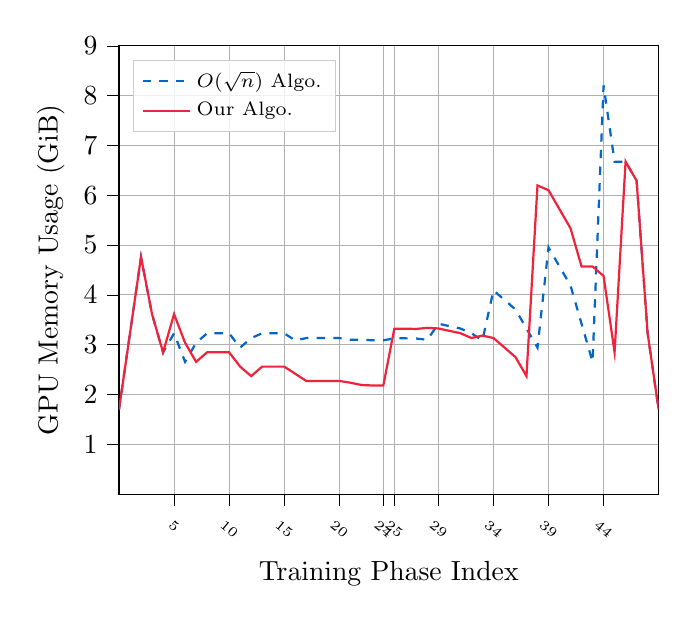
\begin{tikzpicture}

\definecolor{crimson2393560}{RGB}{239,35,60}
\definecolor{darkgray176}{RGB}{176,176,176}
\definecolor{lightgray204}{RGB}{204,204,204}
\definecolor{royalblue4102200}{RGB}{4,102,200}

\begin{axis}[
legend cell align={left},
legend style={fill opacity=0.8, draw opacity=1, text opacity=1, draw=lightgray204},
tick align=outside,
tick pos=left,
title={ },
x grid style={darkgray176},
xlabel={Training Phase Index},
xmajorgrids,
xmin=0, xmax=49,
xtick style={color=black},
xticklabel style={rotate=340.0},
ytick={1,2,3,4,5,6,7,8,9},
xtick={5,10,15,20,24,44,39,34,29,25}, % 3,11,24,46,38,25,
xticklabel style={rotate=340.0, font=\tiny},
legend style={font=\scriptsize},
legend style={at={(0,1)},anchor=north west, xshift=5pt,yshift=-5pt},
y grid style={darkgray176},
ylabel={GPU Memory Usage (GiB)},
ymajorgrids,
ymin=0, ymax=9,
ytick style={color=black}
]
\addplot [thick, royalblue4102200, dashed]
table {%
0 1.69716548919678
1 3.22841548919678
2 4.75966548919678
3 3.61122798919678
4 2.84560298919678
5 3.22841548919678
6 2.65419673919678
7 3.03700923919678
8 3.22841548919678
9 3.22841548919678
10 3.22841548919678
11 2.94130611419678
12 3.13271236419678
13 3.22841548919678
14 3.22841548919678
15 3.22841548919678
16 3.08486080169678
17 3.13271236419678
18 3.13271236419678
19 3.13271236419678
20 3.13271236419678
21 3.09682369232178
22 3.09877681732178
23 3.08876705169678
24 3.08729076385498
25 3.1275634765625
26 3.1270866394043
27 3.1231803894043
28 3.0973014831543
29 3.4202995300293
30 3.3724479675293
31 3.3245964050293
32 3.2288932800293
33 3.0853385925293
34 4.0902214050293
35 3.8988151550293
36 3.7074089050293
37 3.3245964050293
38 2.9417839050293
39 4.9515495300293
40 4.5687370300293
41 4.1859245300293
42 3.4202995300293
43 2.6546745300293
44 8.2054557800293
45 6.6742057800293
46 6.6742057800293
47 6.2913932800293
48 3.2288932800293
49 1.69764280319214
};
\addlegendentry{$O(\sqrt{n})$ Algo.}
\addplot [thick, crimson2393560]
table {%
0 1.69838619232178
1 3.22963619232178
2 4.76088619232178
3 3.61244869232178
4 2.84682369232178
5 3.61244869232178
6 3.03822994232178
7 2.65541744232178
8 2.84682369232178
9 2.84682369232178
10 2.84682369232178
11 2.55971431732178
12 2.36830806732178
13 2.55971431732178
14 2.55971431732178
15 2.55971431732178
16 2.41615962982178
17 2.27260494232178
18 2.27260494232178
19 2.27260494232178
20 2.27260494232178
21 2.23671627044678
22 2.19081783294678
23 2.18080806732178
24 2.17933177947998
25 3.3209228515625
26 3.3204460144043
27 3.3158073425293
28 3.3377799987793
29 3.3258171081543
30 3.2779655456543
31 3.2301139831543
32 3.1344108581543
33 3.1822624206543
34 3.1344108581543
35 2.9430046081543
36 2.7515983581543
37 2.3687858581543
38 6.1969108581543
39 6.1012077331543
40 5.7183952331543
41 5.3355827331543
42 4.5699577331543
43 4.5699577331543
44 4.3785514831543
45 2.8473014831543
46 6.6754264831543
47 6.2926139831543
48 3.2301139831543
49 1.69886350631714
};
\addlegendentry{Our Algo.}
\end{axis}

\end{tikzpicture}

    \caption{GPU Memory Usage: Our Algorithm vs $O(\sqrt{n})$ Memory cost Algorithm Proposed by Chen et al. on VGG-19} 
    \label{fig:our_algo_vs_sublinear}
\end{figure}

In Figure~\ref{fig:our_algo_vs_sublinear}, the red line represents the GPU memory usage of the training on VGG-19 reported by PyTorch using the checkpoint subset returned by our algorithm. On the other hand, the blue dashed line represents the GPU memory usage of the training using the checkpoint subset calculated by the sublinear memory cost algorithm. We mark the ticks of the x-axis using the checkpoint subset of the latter, which is the set \{5, 10, 15, 20, 24\}.

\subsection{Comparison with Optimal Arbitrary Computation Graph Algorithm}

In this experiment, we compare the GPU memory usage when training VGG-19 using the checkpoint subset provided by our algorithm and the one by the optimal arbitrary computation graph algorithm proposed by Feng et al.

\begin{figure}[h!tb]
    \centering
    % This file was created with tikzplotlib v0.10.1.
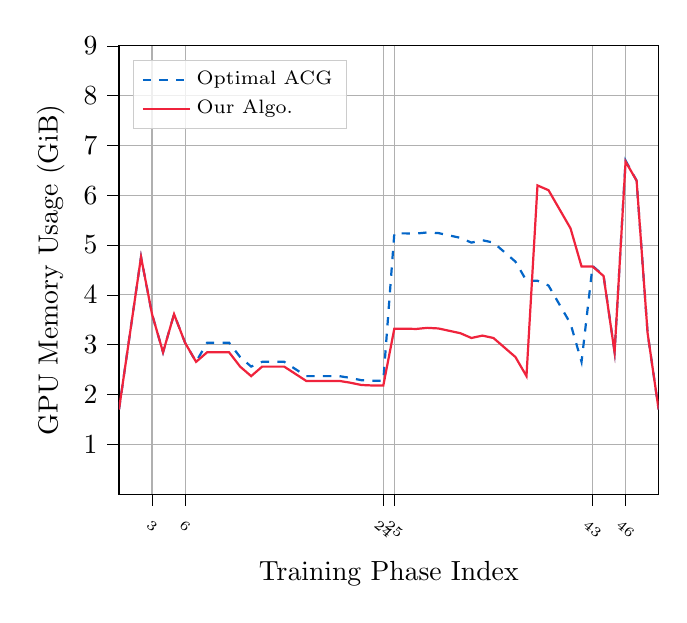
\begin{tikzpicture}

\definecolor{crimson2393560}{RGB}{239,35,60}
\definecolor{darkgray176}{RGB}{176,176,176}
\definecolor{lightgray204}{RGB}{204,204,204}
\definecolor{royalblue4102200}{RGB}{4,102,200}

\begin{axis}[
legend cell align={left},
legend style={fill opacity=0.8, draw opacity=1, text opacity=1, draw=lightgray204},
tick align=outside,
tick pos=left,
title={ },
x grid style={darkgray176},
xlabel={Training Phase Index},
xmajorgrids,
xmin=0, xmax=49,
xtick style={color=black},
xticklabel style={rotate=340.0},
ytick={1,2,3,4,5,6,7,8,9},
xtick={3,6,24,46,43,25},
xticklabel style={rotate=340.0, font=\tiny},
legend style={font=\scriptsize, at={(0,1)},anchor=north west, xshift=5pt,yshift=-5pt},
y grid style={darkgray176},
ylabel={GPU Memory Usage (GiB)},,
ymajorgrids,
ymin=0, ymax=9,
ytick style={color=black}
]
\addplot [thick, royalblue4102200, dashed]
table {%
0 1.69899654388428
1 3.23024654388428
2 4.76149654388428
3 3.61305904388428
4 2.84743404388428
5 3.61305904388428
6 3.03884029388428
7 2.65602779388428
8 3.03884029388428
9 3.03884029388428
10 3.03884029388428
11 2.75173091888428
12 2.56032466888428
13 2.65602779388428
14 2.65602779388428
15 2.65602779388428
16 2.51247310638428
17 2.36891841888428
18 2.36891841888428
19 2.36891841888428
20 2.36891841888428
21 2.33302974700928
22 2.28713130950928
23 2.27712154388428
24 2.27564525604248
25 5.23486328125
26 5.2343864440918
27 5.2312126159668
28 5.2531852722168
29 5.2404899597168
30 5.1926383972168
31 5.1447868347168
32 5.0490837097168
33 5.0969352722168
34 5.0490837097168
35 4.8576774597168
36 4.6662712097168
37 4.2834587097168
38 4.2834587097168
39 4.1877555847168
40 3.8049430847168
41 3.4221305847168
42 2.6565055847168
43 4.5805680847168
44 4.3891618347168
45 2.8579118347168
46 6.6960368347168
47 6.2932243347168
48 3.2307243347168
49 1.69947385787964
};
\addlegendentry{Optimal ACG}
\addplot [thick, crimson2393560]
table {%
0 1.69838619232178
1 3.22963619232178
2 4.76088619232178
3 3.61244869232178
4 2.84682369232178
5 3.61244869232178
6 3.03822994232178
7 2.65541744232178
8 2.84682369232178
9 2.84682369232178
10 2.84682369232178
11 2.55971431732178
12 2.36830806732178
13 2.55971431732178
14 2.55971431732178
15 2.55971431732178
16 2.41615962982178
17 2.27260494232178
18 2.27260494232178
19 2.27260494232178
20 2.27260494232178
21 2.23671627044678
22 2.19081783294678
23 2.18080806732178
24 2.17933177947998
25 3.3209228515625
26 3.3204460144043
27 3.3158073425293
28 3.3377799987793
29 3.3258171081543
30 3.2779655456543
31 3.2301139831543
32 3.1344108581543
33 3.1822624206543
34 3.1344108581543
35 2.9430046081543
36 2.7515983581543
37 2.3687858581543
38 6.1969108581543
39 6.1012077331543
40 5.7183952331543
41 5.3355827331543
42 4.5699577331543
43 4.5699577331543
44 4.3785514831543
45 2.8473014831543
46 6.6754264831543
47 6.2926139831543
48 3.2301139831543
49 1.69886350631714
};
\addlegendentry{Our Algo.}
\end{axis}

\end{tikzpicture}

    \caption{GPU Memory Usage: Our Algorithm vs Optimal Arbitrary Computation Graph (ACG) Algorithm Proposed by Feng et al. on VGG-19} 
    \label{fig:our_algo_vs_optimal_ACG}
\end{figure}

In Figure~\ref{fig:our_algo_vs_optimal_ACG}, the red line represents the GPU memory usage of the training on VGG-19 reported by PyTorch using the checkpoint subset returned by our algorithm. On the other hand, the blue dashed line represents the GPU memory usage of the training using the checkpoint subset returned by the optimal arbitrary computation graph algorithm. We mark the ticks of the x-axis using the checkpoint subset of the latter, which is the set \{3, 6, 24\}.
In the figure, we can see that both algorithms have the same peak memory usage that occurs at the start of the last segment in the backward phase. During the same training phase index range from 25 to 43, the training using the optimal ACG algorithm spends around 2 GiB more memory compared to our algorithm on the first half and more of the first segment during the backward phase. On the other hand, our algorithm also spends around 2 GiB more memory compared to the optimal ACG algorithm on the remaining part of the first segment during the backward phase.

\subsection{Comparison: The Peak Memory Usage on Different Experiment Settings}

\begin{table*}[h!tb]
\centering
\caption{The Profiling Results of Peak Memory Usage: Finding the Checkpoint Subset Using Different Methods}
\label{tab:PR_Peak_Memory_Usage}
\footnotesize
\begin{tabular}{|c|c|c|c|c|c|}
    \hline
    Peak Mem.(MiB) & Algorithm~\ref{alg:dynamic-checkpoint-selection} & Algorithm~\ref{alg:checkpoint-selection} & ACG Solver & $O(\sqrt{n})$ & PyTorch \\
    \hline
    \hline
%    VGG-19, b=128 & {6,444 \{2,4,6,9,11,14,\par 16,19,21,23,24\}} & 6,835 \{3,6,24\} & 6,836 \{3,6,24\} & {8,404 \{5,10,15,\par 20,24\}} & 11,262 \\
    VGG-19, b=128 & 6,444 & 6,835 & 6,836 & 8,404 & 11,262 \\
    & {\{2,4,6,9,11,14,\par 16,19,21,23,24\}} & \{3,6,24\} & \{3,6,24\} & {\{5,10,15,\par 20,24\}} & \\
    \hline
    VGG-19, b=256 & 11,220 & 12,004 & 12,004 & 15,139 & 20,850 \\
    \hline
    VGG-19, b=320 & 13,609 & 14,592 & 14,592 & 18,511 & OOM \\
    \hline
    VGG-19, b=384 & 15,997 & 17,177 & 17,177 & OOM & OOM \\
    \hline
    VGG-19, b=400 & 16,594 & 17,824 & 17,824 & OOM & OOM \\
    \hline
    \hline
%    AlexNet, b=128 & 1,002 \{2,4,6,8\} & 1,003 \{2,4,12,15\} & 1,003 \{2,4,12,15\} & 1,106 \{4,8,12,15\} & 1,174 \\
    AlexNet, b=128 & 1,002 & 1,003 & 1,003 & 1,106 & 1,174 \\
    & \{2,4,6,8,12,14,15\} & \{2,4,12,15\} & \{2,4,12,15\} & \{4,8,12,15\} & \\
    \hline
    AlexNet, b=4096 & 9,866 & 9,866 & 9,866 & 13,182 & 15,275 \\
    \hline
\end{tabular}
\end{table*}

In this experiment, we compare the GPU memory usage when training both VGG-19 and AlexNet with different batch sizes and checkpoint subsets that are computed using different algorithms. The results are shown in Table~\ref{tab:PR_Peak_Memory_Usage}.
In the first column, the shorthand b=$N$ means that we use the number $N$ as the batch size for all experiments of the current row. The abbreviation OOM means that the experiment cannot be carried out due to the out-of-memory error reported by PyTorch.
For the benchmark, we use a single batch from the ImageNet database for testing. (In the implementation of Feng et al., they randomly generate a batch of images for testing.)

For the VGG-19 results in Table~\ref{tab:PR_Peak_Memory_Usage}, both algorithm~\ref{alg:checkpoint-selection} and the optimal ACG algorithm have the same peak memory usage reported by PyTorch since the checkpoint subsets returned by the two algorithms are the same. On the other hand, algorithm~\ref{alg:dynamic-checkpoint-selection} has the lowest peak GPU memory usage. The checkpoint subset returned by algorithm~\ref{alg:checkpoint-selection} and the optimal ACG algorithm is \{3, 6, 24\}. The checkpoint subset returned by algorithm~\ref{alg:dynamic-checkpoint-selection} is \{2, 4, 6, 9, 11, 14, 16, 19, 21, 23, 24\}.
Compared to the $O(\sqrt{n})$ algorithm and ACG Solver, algorithm~\ref{alg:dynamic-checkpoint-selection} reduces 2 GiB (23\%) and 392 MiB (5.7\%) of peak memory usage with a batch size of 128, respectively.
More importantly, the checkpoint subsets do not change when we increase the batch size since the batch size is a factor in the output data size of every layer.

\subsection{The Granularity of Model Specs Matters: Testing The Optimal Checkpoints on AlexNet with Extended Model Specs}

In this subsection, we run Algorithm~\ref{alg:dynamic-checkpoint-selection} on AlexNet model to get the optimal checkpoint subset, and train and profile AlexNet with these checkpoints accordingly. From our prior experiments with VGG-19 models, we observe that the peak GPU memory usage usually occurs at one of the max-pooling layers. But in the plain model specs of AlexNet, all of its max-pooling layers are embedded into {\em larger, abstract} convolution layers, i.e. it is {\em hidden} from the selection of checkpoints. We move all of these max-pooling layers out of the convolution layers since the behavior of our algorithm is dependent on the granularity, i.e. the length, of the model specs. We expect that the peak GPU memory usage will decrease with the new model specs because more combinations are considered.

\subsubsection{AlexNet: Using the Plain Specs}

In this trial, we use the plain model specs of AlexNet, i.e. it has 5 convolution layers and 3 fully-connected layers. The result in Figure~\ref{fig:GMU_AlexNet_Ckpt_Optimal} indicates that our algorithm chose checkpoints \{3, 4, 5, 9, 11, 12\}. This means that the third and fourth convolution layers (Conv2d/ReLU), the fifth convolution layer (Conv2d/ReLU + MaxPool2d), and
%fourth(Conv2d(in=384, out=256), relu, MaxPool2d)  convolution layers
all three fully-connected layers are chosen as checkpoints.

\begin{figure}[h!tb]
\centering

% This file was created with tikzplotlib v0.10.1.
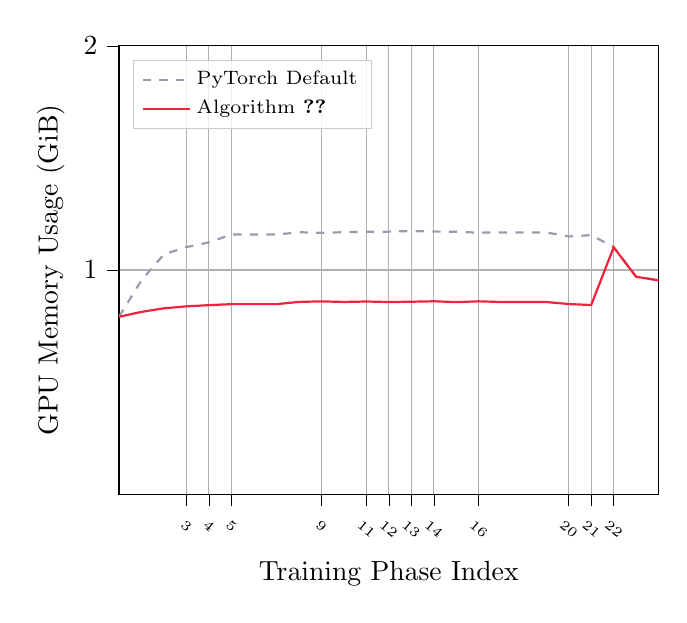
\begin{tikzpicture}

\definecolor{crimson2393560}{RGB}{239,35,60}
\definecolor{darkgray151157172}{RGB}{151,157,172}
\definecolor{darkgray176}{RGB}{176,176,176}
\definecolor{lightgray204}{RGB}{204,204,204}

\begin{axis}[
legend cell align={left},
legend style={fill opacity=0.8, draw opacity=1, text opacity=1, draw=lightgray204},
tick align=outside,
tick pos=left,
title={ },
x grid style={darkgray176},
xlabel={Training Phase Index},
xmajorgrids,
xmin=0, xmax=24,
xtick style={color=black},
xticklabel style={rotate=340.0},
ytick={1,2},
xtick={3,4,5,9,11,12,13,14,16,20,21,22},
xticklabel style={rotate=340.0, font=\tiny},
legend style={font=\scriptsize, at={(0,1)},anchor=north west, xshift=5pt,yshift=-5pt},
y grid style={darkgray176},
ylabel={GPU Memory Usage (GiB)},,
ymajorgrids,
ymin=0, ymax=2,
ytick style={color=black}
]
\addplot [thick, darkgray151157172, dashed]
table {%
0 0.79103125
1 0.95390625
2 1.06978125
3 1.10209375
4 1.12321875
5 1.15784375
6 1.15784375
7 1.15784375
8 1.16834375
9 1.16584375
10 1.16846875
11 1.17046875
12 1.17095703125
13 1.1738837890625
14 1.1712705078125
15 1.1704580078125
16 1.1664580078125
17 1.1673330078125
18 1.1673330078125
19 1.1673330078125
20 1.1493330078125
21 1.1553955078125
22 1.1019580078125
23 0.9702392578125
24 0.9543955078125
};
\addlegendentry{PyTorch Default}
\addplot [thick, crimson2393560]
table {%
0 0.79103125
1 0.81303125
2 0.828875
3 0.83778125
4 0.8430625
5 0.8475625
6 0.8475625
7 0.8475625
8 0.8574375
9 0.85990625
10 0.857328125
11 0.859328125
12 0.85701953125
13 0.8583056640625
14 0.8603173828125
15 0.8565517578125
16 0.8601767578125
17 0.8570517578125
18 0.8570517578125
19 0.8570517578125
20 0.8480517578125
21 0.8435517578125
22 1.1011767578125
23 0.9694580078125
24 0.9536142578125
};
\addlegendentry{Algorithm~\ref{alg:dynamic-checkpoint-selection}}
\end{axis}
\end{tikzpicture}


    \caption{GPU Memory Usage Profiling on Plain AlexNet with The Optimal Set of Checkpoints, \{3, 4, 5, 9, 11, 12\}.} 
    \label{fig:GMU_AlexNet_Ckpt_Optimal}
\end{figure}

\subsubsection{AlexNet: Standalone Max-Pooling Layers}


\begin{figure}[h!tb]
\centering

% This file was created with tikzplotlib v0.10.1.
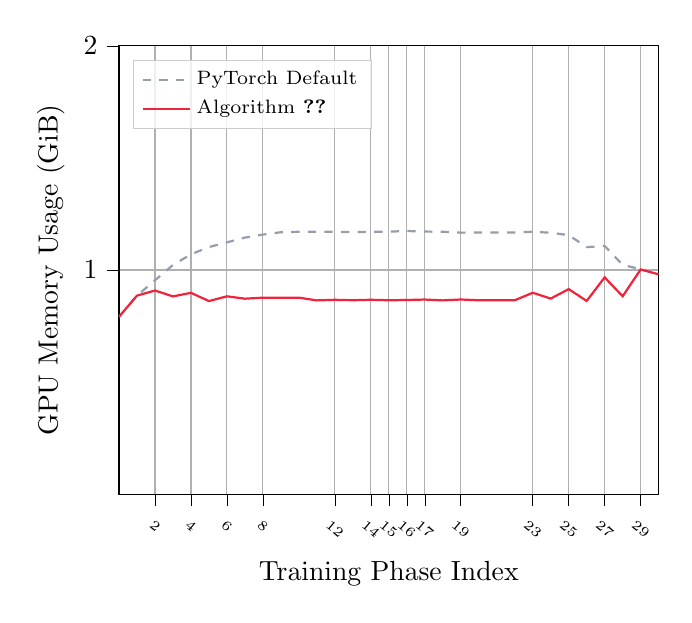
\begin{tikzpicture}

\definecolor{crimson2393560}{RGB}{239,35,60}
\definecolor{darkgray151157172}{RGB}{151,157,172}
\definecolor{darkgray176}{RGB}{176,176,176}
\definecolor{lightgray204}{RGB}{204,204,204}

\begin{axis}[
legend cell align={left},
legend style={fill opacity=0.8, draw opacity=1, text opacity=1, draw=lightgray204},
tick align=outside,
tick pos=left,
title={ },
x grid style={darkgray176},
xlabel={Training Phase Index},
xmajorgrids,
xmin=0, xmax=30,
xtick style={color=black},
xticklabel style={rotate=340.0},
ytick={1,2},
xtick={2,4,6,8,12,14,15,16,17,19,23,25,27,29},
xticklabel style={rotate=340.0, font=\tiny},
legend style={font=\scriptsize, at={(0,1)},anchor=north west, xshift=5pt,yshift=-5pt},
y grid style={darkgray176},
ylabel={GPU Memory Usage (GiB)},,
ymajorgrids,
ymin=0, ymax=2,
ytick style={color=black}
]
\addplot [thick, darkgray151157172, dashed]
table {%
0 0.79103125
1 0.8855625
2 0.95390625
3 1.02225
4 1.06978125
5 1.10209375
6 1.12321875
7 1.14434375
8 1.15784375
9 1.16834375
10 1.17034375
11 1.17034375
12 1.17034375
13 1.16846875
14 1.17046875
15 1.17095703125
16 1.1738837890625
17 1.1712705078125
18 1.1704580078125
19 1.1664580078125
20 1.1673330078125
21 1.1673330078125
22 1.1673330078125
23 1.1704580078125
24 1.1659580078125
25 1.1553955078125
26 1.1019580078125
27 1.1069267578125
28 1.0227392578125
29 1.0033642578125
30 0.9805830078125
};
\addlegendentry{PyTorch Default}
\addplot [thick, crimson2393560]
table {%
0 0.79103125
1 0.88553125
2 0.9083125
3 0.882125
4 0.89796875
5 0.8613125
6 0.8824375
7 0.871875
8 0.876375
9 0.876375
10 0.876375
11 0.86425
12 0.866875
13 0.86503125
14 0.86703125
15 0.86486328125
16 0.8660087890625
17 0.8680205078125
18 0.8642392578125
19 0.8682392578125
20 0.8647392578125
21 0.8647392578125
22 0.8647392578125
23 0.8983173828125
24 0.8723642578125
25 0.9146142578125
26 0.8618017578125
27 0.9668017578125
28 0.8826142578125
29 1.0023330078125
30 0.9805517578125
};
\addlegendentry{Algorithm~\ref{alg:dynamic-checkpoint-selection}}
\end{axis}
\end{tikzpicture}

    \caption{GPU Memory Usage Profiling on Modified AlexNet with The Optimal Set of Checkpoints, \{2, 4, 6, 8, 12, 14, 15\}.} 
    \label{fig:GMU_AlexNet_Ckpt_Optimal2}
\end{figure}

In this trial, we use the extended model specs of AlexNet, i.e. it has 5 convolution layers and 3 standalone max-pooling layers, and 3 fully-connected layers. From the result in Figure~\ref{fig:GMU_AlexNet_Ckpt_Optimal2}, we can see that the checkpoint subset \{2, 4, 6, 8, 12, 14, 15\} is chosen by our algorithm.
%At first look, it might seem that the first checkpoint did not change, but
We should note that since we have changed the granularity of the specs, the numbers (which are indexes) now have a different meaning. It means that the three standalone max-pooling layers (i.e. indices 2, 4, and 8) are chosen as the checkpoints.

In the first convolution layer (Conv2d/ReLU + MaxPool2d) of AlexNet, the output tensor sizes of Conv2d/ReLU and MaxPool2d are 103 MiB and 26 MiB for a batch size of 128, respectively.
Without separating the max-pooling, only the tensor of size 26 MiB can be selected as the checkpoint.
By moving max-pooling out of the layer, the tensor of size 103 MiB becomes a selectable checkpoint.
Consequently, our algorithm identifies a better solution by selecting it as a checkpoint, reducing the peak memory usage by 100 MiB compared to the plain AlexNet model.
The result aligns with our expectations.
We can have a lower peak memory usage if there are more candidates in the model specs as if checkpointing at the middle of an abstract, high-level layer. 

This also shows the advantage of our algorithm. Because the time complexity of our algorithm is linear, the increase in model length caused by the increase in granularity will not affect the speed of our algorithm a lot. (in our cases, there will be at most 7 max-pooling layers given the image size is 224 by 224)



\subsection{Comparison: The Training Time on Different Experiment Settings}

\begin{table*}[h!tb]
\centering
\caption{The Training Time of One Batch Using Different Methods}
\label{tab:training_time}
\footnotesize
\begin{tabular}{|c|c|c|c|c|c|}
    \hline
    Exec. time per batch & Algorithm~\ref{alg:dynamic-checkpoint-selection} & Algorithm~\ref{alg:checkpoint-selection} & ACG Solver & $O(\sqrt{n})$ & PyTorch \\
     (second) & & & & & \\
    \hline
    \hline
%    VGG-19, b=128 & {6,444 \{2,4,6,9,11,14,\par 16,19,21,23,24\}} & 6,835 \{3,6,24\} & 6,836 \{3,6,24\} & {8,404 \{5,10,15,\par 20,24\}} & 11,262 \\
    VGG-19, b=128 & 0.779 & 0.779 & 0.779 & 0.780 & 0.585 \\
    & {\{2,4,6,9,11,14,\par 16,19,21,23,24\}} & \{3,6,24\} & \{3,6,24\} & {\{5,10,15,\par 20,24\}} & \\
    \hline
    VGG-19, b=256 & 1.541 & 1.540 & 1.540 & 1.541 & 1.158 \\
    \hline
    VGG-19, b=320 & 1.921 & 1.920 & 1.920 & 1.922 & OOM \\
    \hline
    VGG-19, b=384 & 2.292 & 2.289 & 2.289 & OOM & OOM \\
    \hline
    VGG-19, b=400 & 2.849 & 2.335 & 2.335 & OOM & OOM \\
    \hline
    \hline
%    AlexNet, b=128 & 1,002 \{2,4,6,8\} & 1,003 \{2,4,12,15\} & 1,003 \{2,4,12,15\} & 1,106 \{4,8,12,15\} & 1,174 \\
    AlexNet, b=128 & 0.046 & 0.046 & 0.046 & 0.046 & 0.038 \\
    & \{2,4,6,8,12,14,15\} & \{2,4,12,15\} & \{2,4,12,15\} & \{4,8,12,15\} & \\
    \hline
    AlexNet, b=4096 & 1.206 & 1.206 & 1.206 & 1.216 & 1.058 \\
    \hline
\end{tabular}
\end{table*}

In this experiment, we compare the training time of VGG-19 and AlexNet with different algorithms.
We train the model for one epoch on the ImageNet dataset and measure the average training time of a single batch.
The results are shown in Table~\ref{tab:training_time}.

For VGG-19, the training time is close with all checkpoint selection methods, irrespective of the number of segments.
The only exception is algorithm~\ref{alg:dynamic-checkpoint-selection} with a batch size of 400, which exhibits 22\% longer time compared to other checkpoint selection methods.
Since this paper focuses on finding the optimal checkpoints with minimal peak memory usage, we will investigate its reason in the future.
Compared with PyTorch, the checkpoint selection methods incur 33\% additional training time with batch sizes of 128 and 256.

As for AlexNet, since AlexNet is a relatively small model, data augmentation becomes a bottleneck and the GPU often becomes idle when waiting for the input data from the CPU.
Therefore, we disable data augmentation and reuse the same input batch data when measuring the training time of AlexNet.
This way avoids extra overhead and ensures full GPU utilization.
The result in Table~\ref{tab:training_time} indicates that the checkpointing methods require 14\% more training time compared to PyTorch with a batch size of 4096.

%For AlexNet, the training time is close with all methods.
%This is because data augmentation is enabled for training, where the augmentation process runs on the CPU.
%Since AlexNet is a relatively small model, this data augmentation becomes a bottleneck, and it often causes the GPU to be idle when waiting for the input data.
%We conduct another experiment without enabling data augmentation and reuse the same input batch data for training AlexNet. This way avoids extra overhead and ensures full GPU utilization. The result indicates that all checkpointing methods require 14\% more training time compared to PyTorch without checkpointing.

We implemented our checkpoint selection algorithms using Python. Algorithm~\ref{alg:checkpoint-selection} and algorithm~\ref{alg:dynamic-checkpoint-selection} respectively take 20 milliseconds and 1.1 milliseconds to find the checkpoint subset for VGG-19, executed on the Intel Xeon Gold 6226R CPU. 